\documentclass[17pt,a4paper,landscape]{extarticle}
\usepackage[margin=2.35cm,top=0.12cm,left=1.05cm]{geometry}
\usepackage{amsmath}
\usepackage{amssymb}
\usepackage{tasks}
\usepackage{tikz}
\usepackage{xcolor}
\usepackage[sfdefault,lf]{FiraSans}
\renewcommand{\familydefault}{\sfdefault}
\setlength{\parindent}{0pt}
\pagestyle{empty}
\settasks{label=\textbf{\arabic*.}, label-width=2.2em, item-indent=2.95em, column-sep=2.1cm, after-item-skip=5.1em}
\renewcommand{\arraystretch}{1.15}
\everymath{\displaystyle}

\newcommand{\threecointree}{%
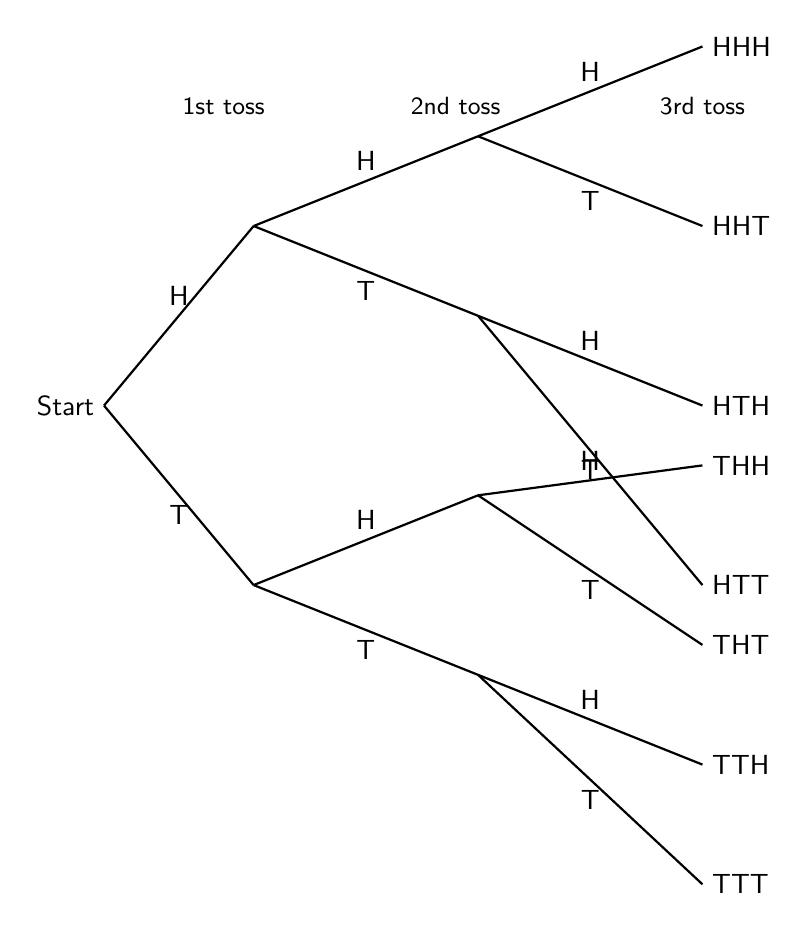
\begin{tikzpicture}[x=0.95cm,y=0.95cm,>=stealth]
  \tikzstyle{branch}=[thick]
  \node[left] at (0,0) {Start};

  \node[font=\small] at (1.6,4.0) {1st toss};
  \node[font=\small] at (4.7,4.0) {2nd toss};
  \node[font=\small] at (8.0,4.0) {3rd toss};

  \draw[branch] (0,0) -- (2,2.4) node[midway,above] {H};
  \draw[branch] (0,0) -- (2,-2.4) node[midway,below] {T};

  \draw[branch] (2,2.4) -- (5,3.6) node[midway,above] {H};
  \draw[branch] (2,2.4) -- (5,1.2) node[midway,below] {T};
  \draw[branch] (2,-2.4) -- (5,-1.2) node[midway,above] {H};
  \draw[branch] (2,-2.4) -- (5,-3.6) node[midway,below] {T};

  \draw[branch] (5,3.6) -- (8,4.8) node[midway,above] {H};
  \draw[branch] (5,3.6) -- (8,2.4) node[midway,below] {T};
  \draw[branch] (5,1.2) -- (8,0.0) node[midway,above] {H};
  \draw[branch] (5,1.2) -- (8,-2.4) node[midway,below] {T};
  \draw[branch] (5,-1.2) -- (8,-0.8) node[midway,above] {H};
  \draw[branch] (5,-1.2) -- (8,-3.2) node[midway,below] {T};
  \draw[branch] (5,-3.6) -- (8,-4.8) node[midway,above] {H};
  \draw[branch] (5,-3.6) -- (8,-6.4) node[midway,below] {T};

  \node[right] at (8,4.8) {HHH};
  \node[right] at (8,2.4) {HHT};
  \node[right] at (8,0.0) {HTH};
  \node[right] at (8,-2.4) {HTT};
  \node[right] at (8,-0.8) {THH};
  \node[right] at (8,-3.2) {THT};
  \node[right] at (8,-4.8) {TTH};
  \node[right] at (8,-6.4) {TTT};
\end{tikzpicture}%
}

\newcommand{\twodicetree}{%
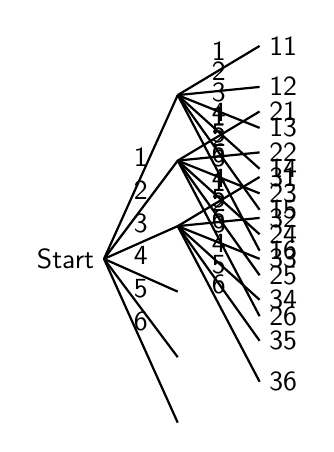
\begin{tikzpicture}[x=0.52cm,y=0.52cm]
  \foreach \y/\n in {4/1,2.4/2,0.8/3,-0.8/4,-2.4/5,-4/6} {
    \draw[thick] (0,0) -- (1.8,\y) node[midway,above] {\n};
  }
  \draw[thick] (1.8,4) -- (3.8,5.2) node[midway,above] {1}; \node[right] at (3.8,5.2) {11};
  \draw[thick] (1.8,4) -- (3.8,4.2) node[midway,above] {2}; \node[right] at (3.8,4.2) {12};
  \draw[thick] (1.8,4) -- (3.8,3.2) node[midway,above] {3}; \node[right] at (3.8,3.2) {13};
  \draw[thick] (1.8,4) -- (3.8,2.2) node[midway,above] {4}; \node[right] at (3.8,2.2) {14};
  \draw[thick] (1.8,4) -- (3.8,1.2) node[midway,above] {5}; \node[right] at (3.8,1.2) {15};
  \draw[thick] (1.8,4) -- (3.8,0.2) node[midway,above] {6}; \node[right] at (3.8,0.2) {16};
  \draw[thick] (1.8,2.4) -- (3.8,3.6) node[midway,above] {1}; \node[right] at (3.8,3.6) {21};
  \draw[thick] (1.8,2.4) -- (3.8,2.6) node[midway,above] {2}; \node[right] at (3.8,2.6) {22};
  \draw[thick] (1.8,2.4) -- (3.8,1.6) node[midway,above] {3}; \node[right] at (3.8,1.6) {23};
  \draw[thick] (1.8,2.4) -- (3.8,0.6) node[midway,above] {4}; \node[right] at (3.8,0.6) {24};
  \draw[thick] (1.8,2.4) -- (3.8,-0.4) node[midway,above] {5}; \node[right] at (3.8,-0.4) {25};
  \draw[thick] (1.8,2.4) -- (3.8,-1.4) node[midway,above] {6}; \node[right] at (3.8,-1.4) {26};
  \draw[thick] (1.8,0.8) -- (3.8,2.0) node[midway,above] {1}; \node[right] at (3.8,2.0) {31};
  \draw[thick] (1.8,0.8) -- (3.8,1.0) node[midway,above] {2}; \node[right] at (3.8,1.0) {32};
  \draw[thick] (1.8,0.8) -- (3.8,0.0) node[midway,above] {3}; \node[right] at (3.8,0.0) {33};
  \draw[thick] (1.8,0.8) -- (3.8,-1.0) node[midway,above] {4}; \node[right] at (3.8,-1.0) {34};
  \draw[thick] (1.8,0.8) -- (3.8,-2.0) node[midway,above] {5}; \node[right] at (3.8,-2.0) {35};
  \draw[thick] (1.8,0.8) -- (3.8,-3.0) node[midway,above] {6}; \node[right] at (3.8,-3.0) {36};
  \node[left] at (0,0) {Start};
\end{tikzpicture}%
}


\begin{document}
\sffamily
\boldmath

\vspace*{0.4em}
{\LARGE \textbf{Excellence}}
\begin{tasks}(2)
\task {Use this tree for Questions 1--4.

\vspace{0.4em}\threecointree}
\task {Is the probability of at least one head equal to $\frac{1}{2}$? Explain.}
\task {Use the tree to find the probability of getting exactly two heads.}
\task {Use the tree to find the probability of getting at least one tail.}
\task {A student says HTH and THH are the same because both have two heads and one tail. Are they correct? Explain using tree paths.}
\task {Use this partial two-dice tree to help find the probability that the total is $7$.

\vspace{0.4em}\twodicetree}
\task {Use the tree to find the probability that both numbers are greater than $4$.}
\task {A spinner has equal sectors labelled A, B, and C. It is spun twice. What is the probability of getting exactly one A?}
\task {A spinner has equal sectors labelled $1$, $2$, $3$, and $4$. It is spun twice. What is the probability that both spins are even?}
\task {A bag has $3$ red and $2$ blue counters. A counter is picked, replaced, then picked again. What is the probability of getting one red and one blue in any order?}
\task {A bag has $3$ red and $2$ blue counters. A counter is picked, replaced, then picked again. What is the probability of getting two counters of the same colour?}
\task {Which is greater: the probability of exactly one head in three coin tosses or the probability of a total of $7$ in two die rolls? Show enough working to justify.}
\task {Which is smaller: the probability of two blues from a bag with $3$ red and $2$ blue counters, with replacement, or the probability of two heads in two coin tosses? Explain.}
\task {Fill in the blank: when a fair coin is tossed three times, the probability of HHH is $\frac{\square}{8}$.}
\task {Fill in the blank: when a fair die is rolled twice, the probability of getting doubles is $\frac{\square}{36}$.}
\task {Which does not belong: outcome, branch, sample space, perimeter? Explain.}
\task {Explain why a full tree diagram helps avoid missing combined outcomes.}
\end{tasks}

\end{document}
